\chapter{طاقة التفاعلات: الاحتراق وطاقات الروابط}\label{ch:g11:reaction-energy}

اكسر ختم مدفأة يد، وبعد دقيقة تصير أسخن من أن تُمسك طويلًا؛ واضغط كيس
تبريد فيبرّد كاحلًا ملتويًا؛ وحافلة مدينة تسير طوال اليوم بالهيدروجين ولا تخلّف
وراءها إلا بخار الماء. فالتحولات الكيميائية لا تحوّل المواد إلى غيرها فحسب: بل
تطلق طاقة، أو تمتصها. فمن أين تأتي هذه الطاقة، وكم منها يستطيع \omterm{def:g4:what-a-fire-needs:fuel}{وقود} أن
يعطي؟

\begin{recall}
في \omterm{def:g8:combustion-and-fuels:complete}{الاحتراق التام}، يحترق \omterm{def:g4:what-a-fire-needs:fuel}{وقود} مكوّن من الكربون والهيدروجين في
ثنائي الأكسجين فيعطي ثنائي أكسيد الكربون والماء
(\cref{ch:g8:combustion-and-fuels}). \omterm{def:g10:lewis-and-shape:covalent-bond}{والرابطة التساهمية} زوج مشترك من
\omterm{def:g9:inside-the-atom:nucleus}{الإلكترونات}؛ وتبيّن صيغ لويس كل روابط \omterm{def:g7:atoms-and-molecules:molecule}{الجزيء}
(\cref{ch:g10:lewis-and-shape}). وتُعدّ \omterm{def:g10:the-mole:amount}{كمية المادة}
\omterm{def:g10:the-mole:amount}{بالمول} (\cref{ch:g10:the-mole}).
\end{recall}

\begin{omfigure}
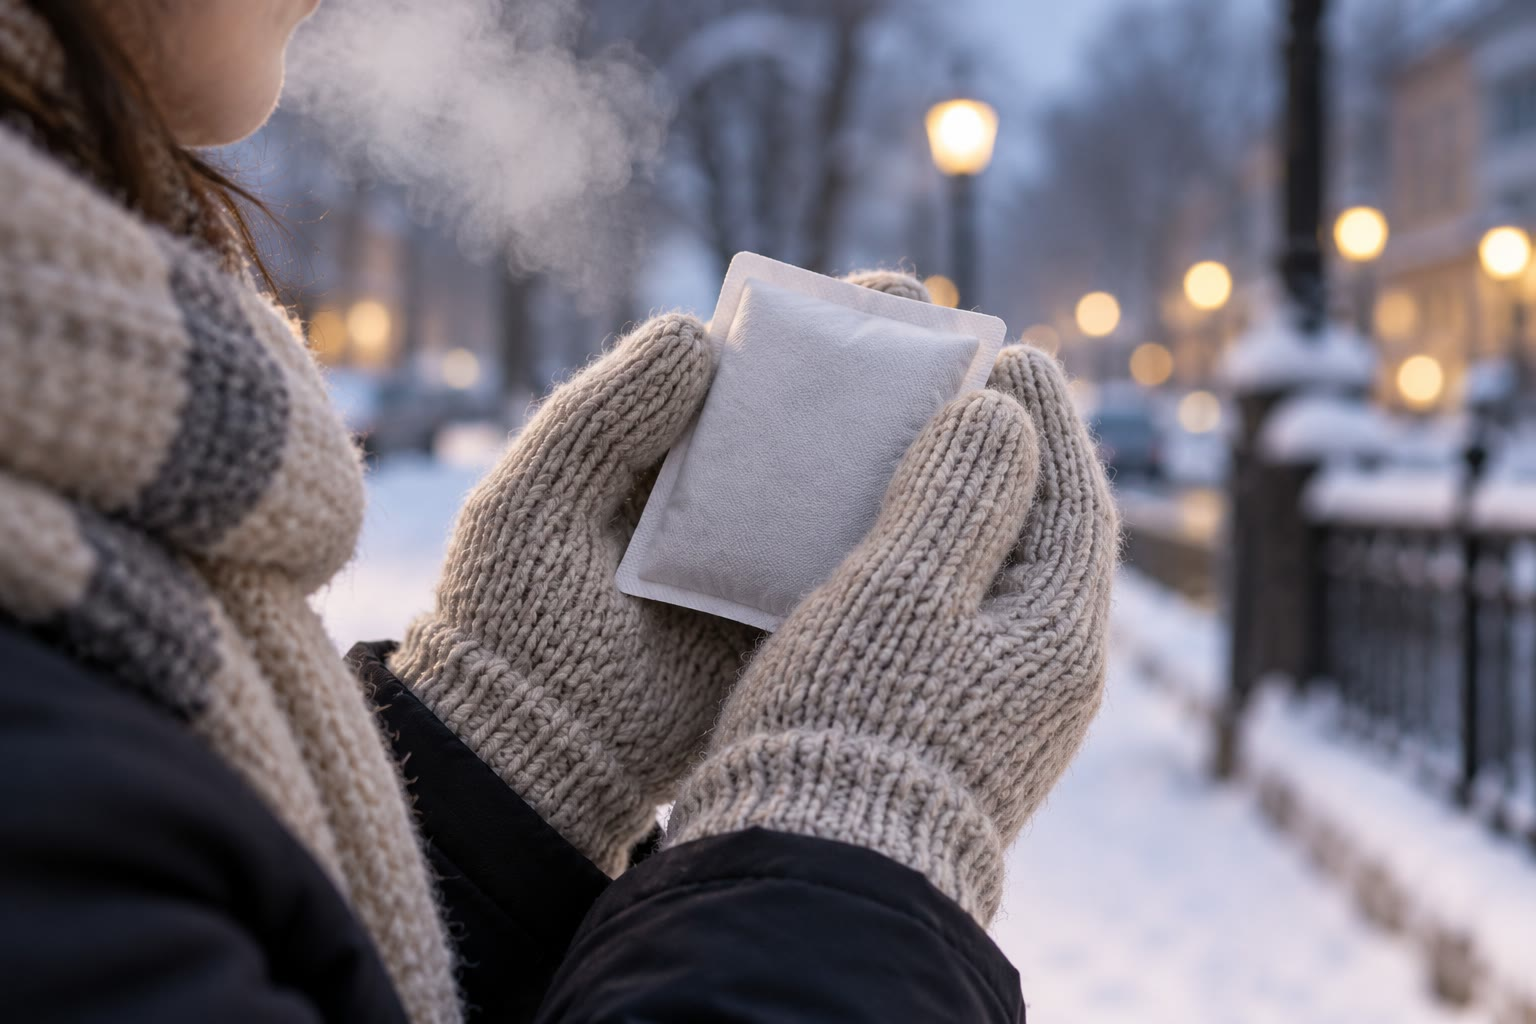
\includegraphics[width=0.45\linewidth]{images/book1/ai/g11-hand-warmers.jpg}

{\small مدفأة يد: تفاعل داخل الكيس يطلق حرارة.}
\end{omfigure}

\section{التحولات الناشرة للحرارة والماصة لها}

\begin{definition}[ناشر للحرارة، ماص للحرارة]\label{def:g11:reaction-energy:exothermic}
يكون التحول \emph{ناشرًا للحرارة}\index{ناشر للحرارة} إذا أطلق
طاقة إلى محيطه، غالبًا على هيئة حرارة: فيسخن المحيط.
ويكون \emph{ماصًا للحرارة}\index{ماص للحرارة} إذا أخذ طاقة من
محيطه: فيبرد المحيط، أو يحتاج التحول إلى التسخين
ليستمر.
\end{definition}

\begin{example}[الساخن والبارد]\label{ex:g11:reaction-energy:packs}
الاحتراقات ناشرة للحرارة، وكذلك التفاعل البطيء لمسحوق الحديد
مع ثنائي أكسجين \omterm{def:g4:air-a-mixture-of-gases:air}{الهواء} داخل مدفأة اليد. \omterm{def:g2:mixing-and-dissolving:dissolve}{وذوبان}
نترات الأمونيوم في الماء، المستعمل في أكياس التبريد، \omterm{def:g11:reaction-energy:exothermic}{ماص للحرارة}؛ وكذلك
تفكك الحجر الجيري إلى جير حي وثنائي أكسيد الكربون، الذي
لا يجري إلا في فرن شديد الحرارة.
\end{example}

\begin{omfigure}
\begin{tikzpicture}[font=\small]
  \begin{scope}
    \draw[->] (0,0) -- (0,3.2) node[above] {الطاقة};
    \draw[very thick, omDef] (0.5,2.5) -- (2.3,2.5) node[right, text=black] {المتفاعلات};
    \draw[very thick, omProp] (0.5,0.8) -- (2.3,0.8) node[right, text=black] {النواتج};
    \draw[->, thick, omThm] (1.4,2.45) -- (1.4,0.85);
    \node[omThm, anchor=west, align=left] at (1.5,1.65) {طاقة\\ محرَّرة};
    \node[anchor=north] at (1.6,-0.15) {\textbf{ناشر للحرارة}};
  \end{scope}
  \begin{scope}[xshift=6cm]
    \draw[->] (0,0) -- (0,3.2) node[above] {الطاقة};
    \draw[very thick, omDef] (0.5,0.8) -- (2.3,0.8) node[right, text=black] {المتفاعلات};
    \draw[very thick, omProp] (0.5,2.5) -- (2.3,2.5) node[right, text=black] {النواتج};
    \draw[->, thick, omDef] (1.4,0.85) -- (1.4,2.45);
    \node[omDef, anchor=west, align=left] at (1.5,1.65) {طاقة\\ ممتصة};
    \node[anchor=north] at (1.6,-0.15) {\textbf{ماص للحرارة}};
  \end{scope}
\end{tikzpicture}

{\small مخططات الطاقة. في التفاعل \omterm{def:g11:reaction-energy:exothermic}{الناشر للحرارة} تختزن \omterm{def:g7:chemical-reactions:reactant}{النواتج} طاقة أقل
من \omterm{def:g7:chemical-reactions:reactant}{المتفاعلات}، ويُطلق الفرق؛ وفي التفاعل \omterm{def:g11:reaction-energy:exothermic}{الماص للحرارة}
تختزن أكثر، ويجب أن يُمدّ به.}
\end{omfigure}

\section{الطاقة التي يطلقها الاحتراق}

\begin{definition}[الطاقة المولية للاحتراق]\label{def:g11:reaction-energy:combustion-energy}
\emph{الطاقة المولية للاحتراق}\index{طاقة مولية للاحتراق}
$E_c$ \omterm{def:g4:what-a-fire-needs:fuel}{لوقود} هي الطاقة التي يطلقها \omterm{def:g8:combustion-and-fuels:complete}{الاحتراق التام} \omterm{def:g10:the-mole:amount}{لمول}
واحد منه، بالوحدة \si{kJ/mol}، والماء المتكوّن سائل.
\end{definition}

\begin{proposition}[الطاقة التي تطلقها $n$ مولات]\label{prop:g11:reaction-energy:n-moles}
% ledger: dch:CH4
يطلق \omterm{def:g8:combustion-and-fuels:complete}{الاحتراق التام} لكمية $n$ من \omterm{def:g4:what-a-fire-needs:fuel}{الوقود} الطاقة
$Q = n \times E_c$. وللميثان $E_c = \qty{890.7}{kJ/mol}$: فحرق
\qty{1.00}{mol} منه (\qty{16.0}{g}) يطلق نحو \qty{891}{kJ}.
\end{proposition}

\begin{proof}
كل \omterm{def:g10:the-mole:amount}{مول} يُحرق من \omterm{def:g4:what-a-fire-needs:fuel}{الوقود} يطلق $E_c$؛ و$n$ مولات تطلق $n$ ضعفًا
من ذلك.
\end{proof}

\begin{inthelab}[تسخين الماء بموقد كحولي]
% ledger: cp:water
يوزن موقد كحولي من الإيثانول، ثم يُشعل تحت علبة معدنية تحوي
\qty{200}{g} من الماء، وفيها مقياس حرارة. وحين يسخن الماء
بمقدار \qty{25}{\celsius}، يُطفأ اللهب ويُوزن الموقد
من جديد: فيكون قد فقد \qty{1.50}{g} من الإيثانول. وتُحسب الطاقة التي أخذها
الماء بعلاقة الفيزياء $Q = m\, c\, \Delta\theta$،
حيث $c = \qty{4.18}{J/(g.\celsius)}$ السعة الحرارية الكتلية للماء. وهي
أدنى بكثير من الطاقة التي يستطيع الإيثانول إطلاقها: فكثير من الحرارة
يسخّن \omterm{def:g4:air-a-mixture-of-gases:air}{الهواء} والعلبة والموقد، وبعض الإيثانول يحترق \omterm{def:g4:what-a-fire-needs:burning}{احتراقًا}
غير تام.
\end{inthelab}

\begin{omfigure}
\begin{tikzpicture}[font=\small]
  % spirit burner
  \fill[black!8, draw=black!60] (-0.6,0) rectangle (0.6,0.7);
  \fill[cyan!15] (-0.55,0.05) rectangle (0.55,0.45);
  \fill[black!40] (-0.06,0.7) rectangle (0.06,0.95);
  \fill[orange!70!yellow] (0,0.95) .. controls (-0.25,1.25) and (-0.1,1.6) .. (0,1.85)
    .. controls (0.1,1.6) and (0.25,1.25) .. (0,0.95);
  \fill[yellow!40] (0,1.0) .. controls (-0.1,1.2) and (-0.05,1.4) .. (0,1.5)
    .. controls (0.05,1.4) and (0.1,1.2) .. (0,1.0);
  % tripod and can
  \draw[black!60, line width=1pt] (-1.1,0) -- (-0.9,2.1) (1.1,0) -- (0.9,2.1);
  \draw[black!60, line width=1.2pt] (-1.1,2.1) -- (1.1,2.1);
  \fill[black!15, draw=black!60] (-0.8,2.1) rectangle (0.8,3.7);
  \fill[omWater] (-0.75,2.15) rectangle (0.75,3.3);
  % thermometer
  \pic at (0.35,2.35) {thermometer};
  \draw[omProp, thick, <-] (0.6,0.35) -- (2.0,0.35) node[right, text=black]
    {موقد كحولي (إيثانول)};
  \draw[omProp, thick, <-] (0.8,2.9) -- (2.0,2.9) node[right, text=black]
    {\foreignlanguage{arabic}{علبة: \qty{200}{g} من الماء}};
  \draw[omProp, thick, <-] (0.45,5.0) -- (2.0,5.0) node[right, text=black]
    {مقياس حرارة};
\end{tikzpicture}

{\small قياس الطاقة التي يعطيها \omterm{def:g4:what-a-fire-needs:fuel}{وقود}: موقد كحولي يسخّن علبة
من الماء يُقاس ارتفاع درجة حرارتها.}
\end{omfigure}


\begin{example}[الموقد الكحولي بالأرقام]\label{ex:g11:reaction-energy:burner}
% ledger: cp:water, dch:C2H5OH, aw:C, aw:H, aw:O
تلقى الماء $Q = 200 \times 4.18 \times 25 = \qty{2.09e4}{J}$،
أي \qty{20.9}{kJ}. والإيثانول المحروق، \qty{1.50}{g}، يساوي
$1.50 / 46.0 = \qty{0.0326}{mol}$؛ ومع $E_c = \qty{1367.6}{kJ/mol}$
كان يستطيع إطلاق $0.0326 \times 1367.6 = \qty{44.6}{kJ}$. ولم يصل إلى الماء
منها إلا $20.9 / 44.6 \approx \qty{47}{\percent}$.
\end{example}

\section{طاقات الروابط}

\begin{definition}[طاقة الرابطة]\label{def:g11:reaction-energy:bond-energy}
\emph{طاقة الرابطة}\index{طاقة الرابطة} التساهمية هي الطاقة
اللازمة لكسر \omterm{def:g10:the-mole:amount}{مول} واحد من هذه الروابط، \omterm{def:g7:atoms-and-molecules:molecule}{والجزيئات} \omterm{def:g7:atoms-and-molecules:atom}{والذرات}
غازية. وتعطي الجداول قيمًا متوسطة، مقيسة على \omterm{def:g7:atoms-and-molecules:molecule}{جزيئات} كثيرة، بالوحدة
\si{kJ/mol}.
\end{definition}

\begin{omfigure}
\small
% ledger: be:H-H, be:C-H, be:N-H, be:O-H, be:H-Cl, be:C-C, be:CC-double, be:C-O, be:CO-double, be:NN-triple, be:OO-double, be:Cl-Cl
\begin{tabular}{lr@{\qquad}lr@{\qquad}lr}
\hline
الرابطة & \si{kJ/mol} & الرابطة & \si{kJ/mol} & الرابطة & \si{kJ/mol} \\
\hline
\ce{H-H} & 436 & \ce{C-C} & 345 & \ce{O=O} & 498 \\
\ce{C-H} & 415 & \ce{C=C} & 611 & \ce{N#N} & 946 \\
\ce{N-H} & 390 & \ce{C-O} & 350 & \ce{Cl-Cl} & 243 \\
\ce{O-H} & 464 & \ce{C=O} & 741 & \ce{H-Cl} & 432 \\
\hline
\end{tabular}\par\medskip

{\small طاقات الروابط المتوسطة. كسر الرابطة يكلّف طاقة دائمًا؛
وتكوينها يعيد الطاقة نفسها.}
\end{omfigure}

\begin{omfigure}
\begin{tikzpicture}[font=\small, x=1cm, y=0.0015cm]
  \draw[->] (0,-850) -- (0,2900) node[above] {\foreignlanguage{arabic}{الطاقة \babelsublr{(\si{kJ})}}};
  \draw[very thick, black!60] (0.4,2656) -- (3.9,2656);
  \node[anchor=west] at (4.0,2656) {\foreignlanguage{arabic}{ذرات منفصلة: \ce{C + 4H + 4O}}};
  \draw[very thick, omDef] (0.4,0) -- (3.9,0);
  \node[anchor=west] at (4.0,0) {\ce{CH4 + 2O2}};
  \draw[very thick, omProp] (0.4,-682) -- (3.9,-682);
  \node[anchor=west] at (4.0,-682) {\ce{CO2 + 2H2O}};
  \draw[->, thick, omDef] (1.0,30) -- (1.0,2626);
  \node[omDef, anchor=west, align=left] at (1.05,1500) {\foreignlanguage{arabic}{كسر \babelsublr{4} \ce{C-H}}\\ \foreignlanguage{arabic}{و\babelsublr{2} \ce{O=O}:}\\ $+\qty{2656}{kJ}$};
  \draw[->, thick, omProp] (3.4,2626) -- (3.4,-652);
  \node[omProp, anchor=west, align=left] at (3.45,1200) {\foreignlanguage{arabic}{تكوين \babelsublr{2} \ce{C=O}}\\ \foreignlanguage{arabic}{و\babelsublr{4} \ce{O-H}:}\\ $-\qty{3338}{kJ}$};
  \draw[<->, omThm, thick] (0.6,-10) -- (0.6,-672);
  \node[omThm, anchor=west] at (0.65,-341) {$E_r \approx \qty{-682}{kJ}$};
\end{tikzpicture}

{\small \omterm{def:g4:what-a-fire-needs:burning}{احتراق} الميثان في خطوتين متخيَّلتين، بطاقات روابط
متوسطة: كسر كل الروابط، ثم تكوين الروابط الجديدة. والتقدير،
\qty{-682}{kJ} لكل \omterm{def:g10:the-mole:amount}{مول} من الميثان، \omterm{def:g11:reaction-energy:exothermic}{ناشر للحرارة}.}
\end{omfigure}

\begin{proposition}[تقدير طاقة التفاعل]\label{prop:g11:reaction-energy:estimate}
لتفاعل بين غازات، تكون الطاقة الممتصة $E_r$ (سالبة إذا
أُطلقت طاقة) تقريبًا
\[
  E_r \approx \sum E(\text{الروابط المكسورة}) - \sum E(\text{الروابط المتكوّنة}) .
\]
فإذا كان $E_r < 0$، كانت الطاقة المطلقة بتكوين الروابط الجديدة أكبر من الطاقة
اللازمة لكسر الروابط القديمة: فالتفاعل \omterm{def:g11:reaction-energy:exothermic}{ناشر للحرارة}.
\end{proposition}

\begin{proof}
تخيّل التفاعل في خطوتين: تُكسر كل روابط \omterm{def:g7:chemical-reactions:reactant}{المتفاعلات}،
وهذا يكلّف المجموع الأول ويترك \omterm{def:g7:atoms-and-molecules:atom}{ذرات} منفصلة؛ ثم تتكوّن روابط
\omterm{def:g7:chemical-reactions:reactant}{النواتج}، وهذا يعيد المجموع الثاني. والنتيجة ليست إلا
تقديرًا، لأن الجداول تعطي متوسطات على \omterm{def:g7:atoms-and-molecules:molecule}{جزيئات} كثيرة.
\end{proof}

\begin{method}[تقدير طاقة التفاعل من طاقات الروابط]\label{met:g11:reaction-energy:bonds}
\begin{enumerate}
  \item اكتب \omterm{def:g8:balanced-equations:equation}{المعادلة الموزونة} وصيغة لويس لكل
        \omterm{def:g7:atoms-and-molecules:molecule}{جزيء}.
  \item عُدّ الروابط من كل نوع المكسورة في \omterm{def:g7:chemical-reactions:reactant}{المتفاعلات} والمتكوّنة
        في \omterm{def:g7:chemical-reactions:reactant}{النواتج}، مع المعاملات.
  \item اجمع طاقات الروابط المكسورة، واطرح منها طاقات
        الروابط المتكوّنة.
  \item استنتج: النتيجة السالبة تعني تفاعلًا \omterm{def:g11:reaction-energy:exothermic}{ناشرًا للحرارة}.
\end{enumerate}
\end{method}

\begin{example}[الهيدروجين والكلور]\label{ex:g11:reaction-energy:hcl}
% ledger: be:H-H, be:Cl-Cl, be:H-Cl
للتفاعل \ce{H2 + Cl2 -> 2HCl}: تُكسر رابطة \ce{H-H} واحدة ورابطة \ce{Cl-Cl} واحدة،
$436 + 243 = \qty{679}{kJ}$؛ وتتكوّن رابطتا \ce{H-Cl}، $2 \times 432 =
\qty{864}{kJ}$. إذن $E_r \approx 679 - 864 = \qty{-185}{kJ}$ لكل \omterm{def:g10:the-mole:amount}{مول} من
التفاعل: \omterm{def:g11:reaction-energy:exothermic}{ناشر للحرارة}.
\end{example}


\begin{remark}[التقدير والقياس]\label{rem:g11:reaction-energy:compare}
% ledger: dch:CH4
الطاقة المقيسة التي يطلقها حرق \omterm{def:g10:the-mole:amount}{مول} واحد من الميثان
\qty{890.7}{kJ}، وهي أكبر من التقدير. ولذلك ثلاثة أسباب: روابط \ce{C=O}
في ثنائي أكسيد الكربون أقوى من الرابطة \ce{C=O} المتوسطة في
الجدول؛ والقيمة المقيسة تخص الماء السائل، وتكاثف بخار
الماء يطلق طاقة إضافية؛ وطاقات الروابط المتوسطة ليست إلا
متوسطات. فطريقة طاقات الروابط تعطي الإشارة ورتبة
المقدار، لا القيمة الدقيقة.
\end{remark}

\section{مقارنة أنواع الوقود}

\begin{omfigure}
\begin{tikzpicture}
\begin{axis}[xbar, width=0.78\linewidth, height=5.4cm, xmin=0, xmax=160,
    xlabel={\foreignlanguage{arabic}{الطاقة المطلقة لكل كيلوغرام محروق \babelsublr{(\si{MJ/kg})}}},
    symbolic y coords={ethanol, octane, propane, methane, hydrogen},
    yticklabels={{الإيثانول}, {الأوكتان}, {البروبان}, {الميثان}, {الهيدروجين}},
    ytick=data, bar width=10pt, nodes near coords,
    nodes near coords style={font=\footnotesize, /pgf/number format/fixed,
      /pgf/number format/precision=1, /pgf/number format/fixed zerofill},
    tick label style={font=\small}, label style={font=\small},
    axis lines*=left, xmajorgrids, grid style={gray!20}, enlarge y limits=0.15]
  % ledger: dch:C2H5OH, dfh:C8H18, dfh:CO2, dfh:H2O-l, dch:C3H8, dch:CH4 (per kg with the book's molar masses)
  \addplot[fill=omProp!55, draw=omProp] coordinates {(29.7,ethanol) (48.0,octane)
    (50.4,propane) (55.7,methane) (142.9,hydrogen)};
\end{axis}
\end{tikzpicture}

{\small الطاقة التي يطلقها \omterm{def:g8:combustion-and-fuels:complete}{الاحتراق التام} لكيلوغرام واحد من خمسة أنواع
من \omterm{def:g4:what-a-fire-needs:fuel}{الوقود} (والماء المتكوّن سائل). يعطي الهيدروجين أكثرها بفارق كبير
لكل كيلوغرام؛ والإيثانول، وهو «محترق» جزئيًا من قبل (فهو يحوي الأكسجين)،
أقلها.}
\end{omfigure}

\begin{example}[ثنائي أكسيد الكربون لكل ميغاجول]\label{ex:g11:reaction-energy:co2}
% ledger: dch:CH4, dch:C2H5OH
يطلق حرق \omterm{def:g10:the-mole:amount}{مول} واحد من الميثان \qty{890.7}{kJ} ومولًا واحدًا من
ثنائي أكسيد الكربون، \qty{44.0}{g}. فلكل ميغاجول، أي \qty{1000}{kJ}، يطلق
$44.0 \times 1000 / 890.7 = \qty{49.4}{g}$ من ثنائي أكسيد الكربون.
أما الإيثانول، بمولين من ثنائي أكسيد الكربون لكل \qty{1367.6}{kJ}، فيطلق
$88.0 \times 1000 / 1367.6 = \qty{64.3}{g}$ لكل ميغاجول. والهيدروجين
لا يطلق شيئًا منه: فناتجه الوحيد الماء.
\end{example}

\begin{omfigure}
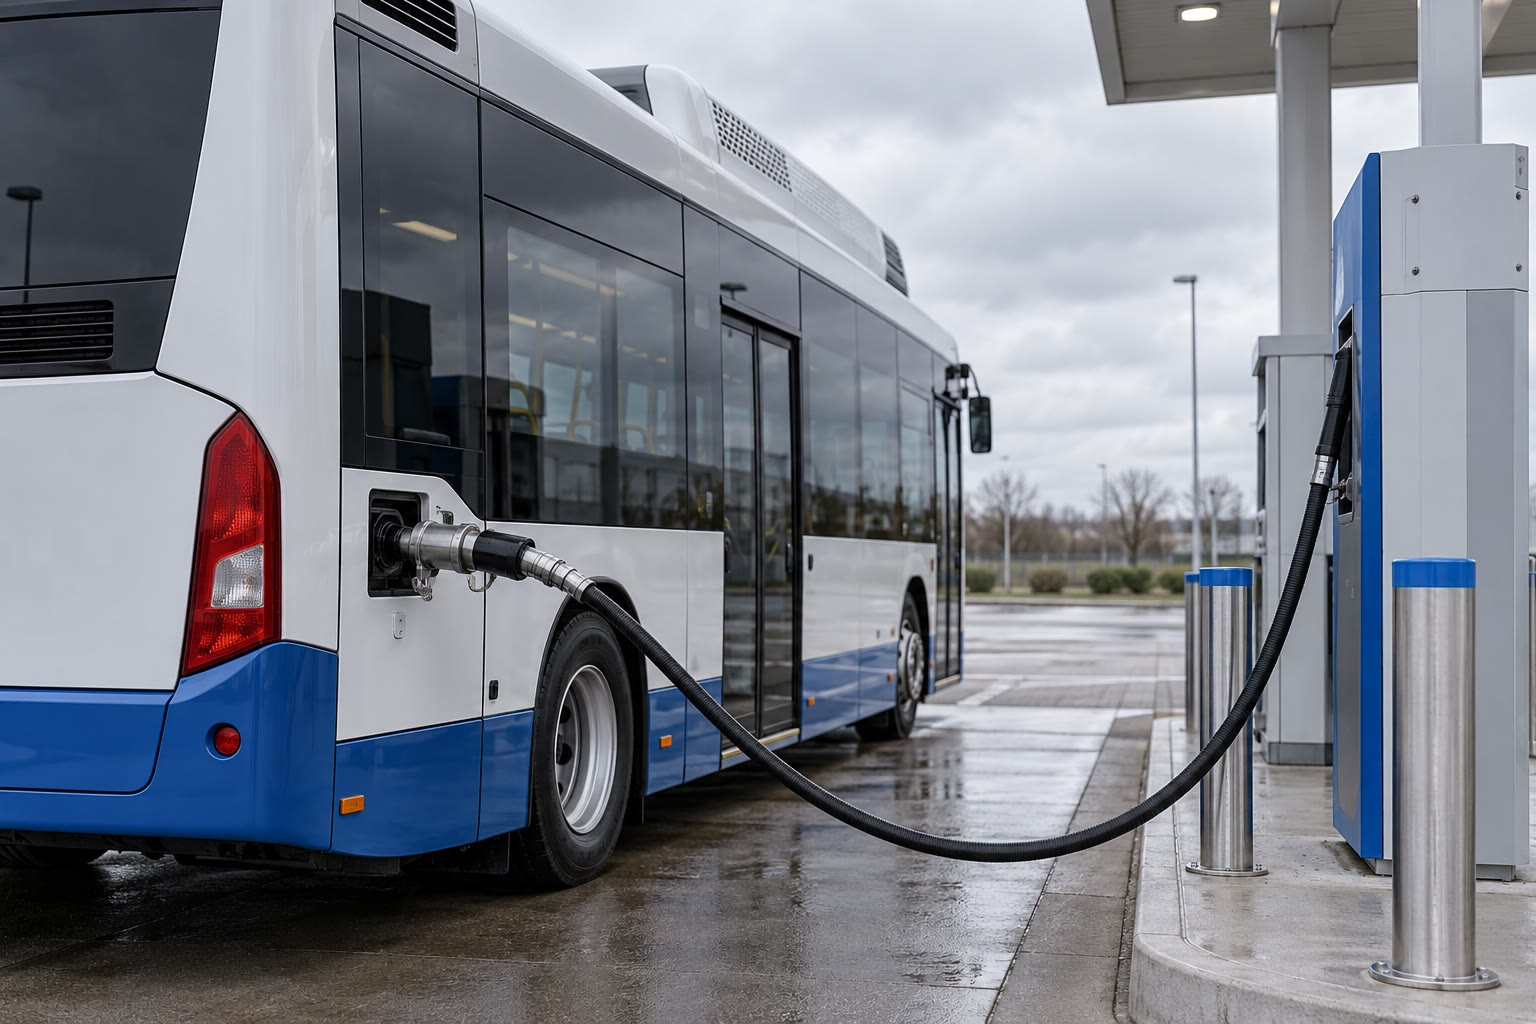
\includegraphics[width=0.5\linewidth]{images/book1/ai/g11-hydrogen-bus.jpg}

{\small حافلة في محطة هيدروجين: وقودها لا يطلق إلا الماء.}
\end{omfigure}

\begin{safety}{\ghs[0.82cm]{GHS02}\ghs[0.82cm]{GHS07}}
% ledger: ghs:ethanol
الإيثانول شديد القابلية للاشتعال ومهيّج للعينين. ويُملأ الموقد الكحولي
بعيدًا عن أي لهب، ولا يُعاد ملؤه وهو ساخن، ولا يستعمله إلا
المعلم على حصيرة مقاومة للحرارة.
\end{safety}

\section{تمارين}


\begin{exercise}[$\star$]\label{exo:g11:reaction-energy:1}
\omterm{def:g11:reaction-energy:exothermic}{ناشر للحرارة} أم ماص لها: \omterm{def:g4:what-a-fire-needs:burning}{احتراق} الخشب؛ انصهار الجليد؛ ضغط كيس
تبريد؛ تسخّن مدفأة يد؛ صنع ورقة خضراء للسكر في
ضوء الشمس؟
\end{exercise}

\begin{exercise}[$\star$]\label{exo:g11:reaction-energy:2}
% ledger: dch:CH4
ما الطاقة التي يطلقها \omterm{def:g8:combustion-and-fuels:complete}{الاحتراق التام} لكمية \qty{3.0}{mol} من الميثان؟
\end{exercise}

\begin{exercise}[$\star$]\label{exo:g11:reaction-energy:3}
في مخطط الطاقة لتفاعل \omterm{def:g11:reaction-energy:exothermic}{ناشر للحرارة}، أيهما يختزن طاقة
أكثر، \omterm{def:g7:chemical-reactions:reactant}{المتفاعلات} أم \omterm{def:g7:chemical-reactions:reactant}{النواتج}؟ وإلى أين يذهب الفرق؟
\end{exercise}

\begin{exercise}[$\star$]\label{exo:g11:reaction-energy:4}
% ledger: dch:C2H5OH
ما الطاقة التي يطلقها \omterm{def:g8:combustion-and-fuels:complete}{الاحتراق التام} لكتلة \qty{100}{g} من الإيثانول؟
\end{exercise}

\begin{exercise}[$\star$]\label{exo:g11:reaction-energy:5}
ما \omterm{def:g11:reaction-energy:bond-energy}{طاقة الرابطة}؟ ولماذا يكلّف كسر الرابطة طاقة دائمًا؟
\end{exercise}

\begin{exercise}[$\star\star$]\label{exo:g11:reaction-energy:6}
قدّر، بطاقات الروابط، طاقة التفاعل
\ce{2H2 + O2 -> 2H2O}، والأنواع كلها غازية. أهو \omterm{def:g11:reaction-energy:exothermic}{ناشر للحرارة}؟
\end{exercise}

\begin{exercise}[$\star\star$]\label{exo:g11:reaction-energy:7}
قدّر طاقة \omterm{def:g4:what-a-fire-needs:burning}{احتراق} الإيثانول، \ce{C2H5OH + 3O2 ->
2CO2 + 3H2O}، بطاقات الروابط (ارسم صيغة لويس للإيثانول
أولًا)، وقارنها بالقيمة المقيسة \qty{1367.6}{kJ/mol}.
\end{exercise}

\begin{exercise}[$\star\star$]\label{exo:g11:reaction-energy:8}
% ledger: dch:C3H8, dch:CH4
احسب الطاقة المطلقة لكل كيلوغرام من البروبان
(\qty{2219.2}{kJ/mol}) ومن الميثان. وقارن بالمخطط الشريطي.
\end{exercise}

\begin{exercise}[$\star\star$]\label{exo:g11:reaction-energy:9}
% ledger: cp:water, dch:CH4
يسخّن موقد غاز \qty{1.50}{L} من الماء (\qty{1500}{g}) من
\qty{15}{\celsius} إلى \qty{100}{\celsius}. ما الطاقة التي يتلقاها
الماء؟ وما كتلة الميثان المحروقة إذا وصلت الطاقة كلها إلى
الماء؟ وإذا لم يصل إلا نصفها؟
\end{exercise}

\begin{exercise}[$\star\star$]\label{exo:g11:reaction-energy:10}
مستعينًا بالمخطط الشريطي، رتّب أنواع \omterm{def:g4:what-a-fire-needs:fuel}{الوقود} بحسب الطاقة لكل كيلوغرام. وما كتلة
الهيدروجين التي تعطي الطاقة نفسها التي يعطيها \qty{1.0}{kg} من الأوكتان؟
\end{exercise}

\begin{exercise}[$\star\star$]\label{exo:g11:reaction-energy:11}
قدّر طاقة التفاعل \ce{N2 + 3H2 -> 2NH3}، والأنواع كلها غازية. أهو \omterm{def:g11:reaction-energy:exothermic}{ناشر للحرارة} أم
ماص لها؟
\end{exercise}

\begin{exercise}[$\star\star\star$]\label{exo:g11:reaction-energy:12}
% ledger: cp:water, dch:C2H5OH
في تجربة موقد كحولي، يسخن \qty{250}{g} من الماء بمقدار
\qty{20}{\celsius} بينما يحترق \qty{1.20}{g} من الإيثانول. احسب
الطاقة التي تلقاها الماء، والطاقة التي يستطيع الإيثانول إطلاقها،
ومردود التسخين. واذكر ثلاثة أسباب للضياع.
\end{exercise}

\begin{exercise}[$\star\star\star$]\label{exo:g11:reaction-energy:13}
% ledger: dfh:C8H18, dfh:CO2, dfh:H2O-l, dch:C3H8
يطلق الأوكتان \qty{5470}{kJ/mol} والبروبان \qty{2219.2}{kJ/mol}.
اكتب معادلتي احتراقهما واحسب كتلة ثنائي أكسيد الكربون
التي يطلقها كل منهما لكل ميغاجول. وقارن بالميثان، \qty{49.4}{g}.
\end{exercise}

\begin{exercise}[$\star\star\star$]\label{exo:g11:reaction-energy:14}
للميثان والإيثانول كليهما، تقدير طاقات الروابط أصغر من
الطاقة المطلقة المقيسة. أعطِ الأسباب، واشرح لماذا يبقى
التقدير مفيدًا.
\end{exercise}

\begin{exercise}[$\star\star\star$]\label{exo:g11:reaction-energy:15}
قدّر طاقة التفاعل \ce{2H2O -> 2H2 + O2}، والأنواع كلها غازية. لماذا يجب
إمداد الطاقة (مثلًا على هيئة كهرباء) لصنع الهيدروجين من الماء؟
واشرح لماذا يُسمّى الهيدروجين وسيلةً \emph{لتخزين} الطاقة لا
مصدرًا لها.
\end{exercise}

\section{مسألة: أي وقود لحافلة المدينة؟}

\begin{problem}[{مسألة نهاية الأسبوع --- الميثان أم الإيثانول أم الأوكتان أم الهيدروجين:
أيها يعطي أكبر طاقة لكل كيلوغرام، وكم من ثنائي أكسيد الكربون لكل
ميغاجول؟}]
\label{pb:g11:reaction-energy:1}
% ledger: dch:CH4, dch:C2H5OH, dfh:C8H18, dfh:CO2, dfh:H2O-l, be:C-H, be:OO-double, be:CO-double, be:O-H
تقارن مدينة بين أربعة أنواع من \omterm{def:g4:what-a-fire-needs:fuel}{الوقود} لحافلاتها: الميثان (الغاز الطبيعي)، والإيثانول،
والأوكتان (للبنزين) والهيدروجين. والطاقات التي يطلقها \omterm{def:g8:combustion-and-fuels:complete}{الاحتراق
التام} \omterm{def:g10:the-mole:amount}{لمول} واحد هي: الميثان \qty{890.7}{kJ}، والإيثانول
\qty{1367.6}{kJ}، والأوكتان \qty{5470}{kJ}، والهيدروجين \qty{285.8}{kJ}،
والماء المتكوّن سائل.

\medskip
\noindent\textbf{الجزء الأول --- معادلات \omterm{def:g4:what-a-fire-needs:burning}{الاحتراق}.}
\begin{enumerate}
  \item اكتب معادلة \omterm{def:g8:combustion-and-fuels:complete}{الاحتراق التام} للميثان.
  \item ثم للإيثانول، \ce{C2H6O}.
  \item ثم للأوكتان، \ce{C8H18}.
  \item ثم للهيدروجين.
  \item أي \omterm{def:g4:what-a-fire-needs:fuel}{وقود} لا يطلق ثنائي أكسيد الكربون؟
\end{enumerate}

\medskip
\noindent\textbf{الجزء الثاني --- الطاقة لكل كيلوغرام.}
\begin{enumerate}[resume]
  \item احسب الكتل المولية لأنواع \omterm{def:g4:what-a-fire-needs:fuel}{الوقود} الأربعة.
  \item احسب الطاقة المطلقة لكل كيلوغرام لكل منها، بالوحدة
        \si{MJ/kg}.
  \item رتّب أنواع \omterm{def:g4:what-a-fire-needs:fuel}{الوقود}.
  \item يفوز الهيدروجين بفارق كبير. فلماذا يبقى حمله على
        حافلة صعبًا؟ (فكّر في حالته عند درجة حرارة الغرفة.)
\end{enumerate}

\medskip
\noindent\textbf{الجزء الثالث --- التقدير بطاقات الروابط.}
\begin{enumerate}[resume]
  \item ارسم صيغ لويس \omterm{def:g7:atoms-and-molecules:molecule}{لجزيئات} \omterm{def:g4:what-a-fire-needs:burning}{احتراق}
        الميثان، وعُدّ الروابط المكسورة والمتكوّنة.
  \item احسب الطاقة اللازمة لكسر الروابط.
  \item احسب الطاقة المطلقة بتكوين الروابط الجديدة.
  \item استنتج تقدير $E_r$، وقارنه بالقيمة
        المقيسة: ما الفرق النسبي؟
  \item أعطِ سببين للفرق.
\end{enumerate}

\medskip
\noindent\textbf{الجزء الرابع --- ثنائي أكسيد الكربون لكل ميغاجول.}
\begin{enumerate}[resume]
  \item ما كمية الميثان التي يجب أن تحترق لإطلاق \qty{1}{MJ}؟
  \item ما كتلة ثنائي أكسيد الكربون التي تطلقها؟
  \item السؤال نفسه للإيثانول والأوكتان.
  \item أي \omterm{def:g4:what-a-fire-needs:fuel}{وقود} كربوني يطلق أقل قدر من ثنائي أكسيد الكربون للطاقة
        نفسها؟ ولماذا (قارن أعداد \omterm{def:g7:atoms-and-molecules:atom}{ذرات} C وH)؟
  \item لا يطلق الهيدروجين شيئًا منه حين يحترق. فعلامَ تتوقف
        فائدته الحقيقية للمناخ؟
  \item اذكر الجواب النهائي: ما كتلة ثنائي أكسيد الكربون التي يطلقها الميثان
        لكل ميغاجول؟
\end{enumerate}
\end{problem}
